\begin{minipage}{0.63\linewidth}
On produit à l'aide d'une plaque $(P)$ d'un vibreur, à la surface libre de l'eau
d'une cuve à ondes, des ondes progressives périodiques de fréquence
$N=\qty{10}{\hertz}$. Les ondes se propagent sans amortissement ni réflexion. La
figure~\ref{fig:cuve_surface_eau} donne l'aspect de la surface de l'eau à un
instant donné.

\textbf{Donnée~:} $d=\qty{6}{\cm}$.
\begin{enumerate}
    \item Déterminer la valeur de la longueur d'onde $\lambda$.
    \item Déduire la valeur de la vitesse de propagation $v$ à la surface de
          l'eau.
    \item On considère deux points $M$ et $P$ de la surface de l'eau, tel que
          $MP=\qty{7}{\cm}$ (figure~\ref{fig:cuve_surface_eau}). Calculer le
          retard temporel $\tau$ de la vibration du point $P$ par rapport à $M$.
\end{enumerate}
\end{minipage}
\hfill
\begin{minipage}{0.36\linewidth}
    \begin{figure}[H]
        \centering
        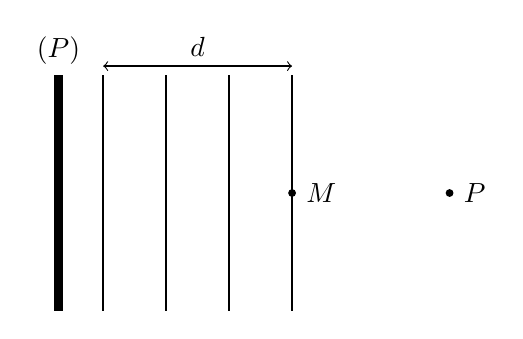
\begin{tikzpicture}
            \node[fill,inner sep=0pt,minimum width=1.2mm,
                minimum height=3cm,label=$(P)$] (P) {};
            \foreach \x [count=\i] in {0.5,1.3,2.1,...,3}
            \node[fill,inner sep=0pt,minimum width=1pt,
                minimum height=3cm] (n\i) at ([xshift=\x cm]P.east) {};
            \draw[<->] ([yshift=3pt]n1.north) --
                node[above] {$d$} ([yshift=3pt]n4.north);
            \foreach \l/\p in {M/0,P/2}
            \node[circle,fill,inner sep=1pt,
                label=right:$\l$] at ([xshift=\p cm]n4.center) {};
        \end{tikzpicture}
        \caption{}
        \label{fig:cuve_surface_eau}
    \end{figure}
\end{minipage}

